\documentclass{article}
\usepackage{algorithm}
\usepackage{algpseudocode}
\usepackage{graphicx}
\usepackage{geometry}

\title{Algoritmi - Lezione 2}
\author{Ionut Zbirciog}
\date{10 October 2023}

\begin{document}
\maketitle

\

\section{Modelli di Calcolo}

\subsection{Macchina di Turing}
\begin{figure}[h]
  \centering
  \includegraphics[width=0.4\textwidth]{turing.png}
  \caption{Macchina di Turing.}
\end{figure}
\begin{itemize}
    \item Troppo di basso livello.
    \item Utile per calcoli ma poco efficiente.
\end{itemize}

\subsection{Modello RAM (Random Access Machine)}
\begin{figure}[h]
  \centering
  \includegraphics[width=0.4\textwidth]{RAM.png}
  \caption{Modello di Von Neumann.}
\end{figure}
\begin{itemize}
    \item Un programma finito.
    \item Un nastro di input e uno di output.
    \item Una memoria strutturata come un array.
    \item Una CPU per eseguire istruzioni.
\end{itemize}

\subsection{Analisi della Complessità di Algoritmi}
L'analisi della complessità di un algoritmo si basa sul concetto di passo elementare. I passi elementari su una RAM includono:
\begin{itemize}
    \item Istruzione I/O.
    \item Operazione aritmetica/logica.
    \item Accesso/modifica della memoria.
\end{itemize}

\section{Criteri di Costo}

\subsection{Criterio di Costo Uniforme}
È generalmente usato e assume che tutte le operazioni abbiano lo stesso costo. La complessità temporale è misurata come il numero di passi elementari eseguiti.

\subsection{Criterio di Costo Logaritmico}
Il costo di un'operazione dipende dagli operandi. Un'operazione su un operando $x$ ha costo $\log(x)$. Questo criterio modella meglio la complessità di algoritmi numerici.

\section{Caso Peggiore}

Si definisce il tempo di esecuzione $T(I)$ di un algoritmo sull'istanza $I$. $T_{\text{worst}}(n)$ rappresenta il tempo di esecuzione sulle istanze di ingresso che comportano più lavoro per l'algoritmo. Questo fornisce una garanzia sul tempo di esecuzione per ogni istanza.
\\
$T_{\text{worst}}(n) = \max_{I \text{ dim } n} \{\text{tempo}(I)\}$

\section{Caso Medio}

Sia $P(I)$ la probabilità di occorrenza dell'istanza $I$. $T_{\text{avg}}(n)$ rappresenta il tempo di esecuzione nel caso medio, cioè sulle istanze di ingresso tipiche per il problema. Poiché non è sempre possibile conoscere la distribuzione di probabilità sulle istanze, si fanno delle assunzioni.
\\
$T_{\text{avg}}(n) = \sum_{I \text{ dim } n} \{P(I) \cdot \text{tempo}(I)\}$

\section{Notazione Asintotica}
$T(n)$ = numero di passi elementari eseguiti su una RAM nel caso peggire su un'istanza di dimensione n.
Si utilizza la notazione asintotica per descrivere la complessità di un algoritmo in modo qualitativo, ignorando costanti moltiplicative e termini di ordine inferiore. L'assunzione implicita è che stiamo considerando istanze di grandi dimensioni.

\subsection{Notazione \textit{O} Grande}
Definiamo $f(n) = O(g(n))$ se esistono due costanti $c > 0$ e $n_0 > 0$ tali che $0 \leq f(n) \leq c \cdot g(n)$ per ogni $n \geq n_0$.
\begin{figure}[h]
  \centering
  \includegraphics[width=0.4\textwidth]{O.png}
\end{figure}
\\  
Esempi:
\begin{align}
    f(n) &= 2n^2 + 3n \\
    f(n) &= O(n^3) \\
    f(n) &= O(n^2) \\
    f(n) &\neq O(n)
\end{align}
\\\\
\textbf{Nota:} \\
$\lim_{n\to\infty} \frac{f(n)}{g(n)} = 0 \Rightarrow f(n) = O(g(n))$ \\
$f(n) = O(g(n)) \not\Rightarrow \lim_{n\to 0} \frac{f(n)}{g(n)} = 0$ \\
$f(n) = O(g(n)) \Rightarrow \lim_{n\to\infty} \frac{f(n)}{g(n)}$ (se esiste) $< \infty$
\\\\\\
\subsection{Notazione Omega Grande}
Definiamo $f(n) = \Omega(g(n))$ se esistono due costanti $c > 0$ e $n_0 > 0$ tali che $f(n) \geq c \cdot g(n) \geq 0$ per ogni $n \geq n_0$.
\begin{figure}[h]
  \centering
  \includegraphics[width=0.4\textwidth]{Omega.png}
\end{figure}
\\
Esempi:
\begin{align}
    f(n) &= 2n^2 - 3n \\
    f(n) &= \Omega(n) \\
    f(n) &= \Omega(n^2) \\
    f(n) &\neq \Omega(n^3)
\end{align}
\\\\
\textbf{Nota:} \\
$\lim_{n\to\infty} \frac{f(n)}{g(n)} = \infty \Rightarrow f(n) = \Omega(g(n))$ \\
$f(n) = \Omega(g(n)) \not\Rightarrow \lim_{n\to 0} \frac{f(n)}{g(n)} = \infty$ \\
$f(n) = O(g(n)) \Rightarrow \lim_{n\to\infty} \frac{f(n)}{g(n)}$ (se esiste) $> 0$


\subsection{Notazione Theta}
Definiamo $f(n) = \Theta(g(n))$ se esistono tre costanti $c_1 > 0$, $c_2 > 0$, e $n_0 > 0$ tali che $c_1 \cdot g(n) \leq f(n) \leq c_2 \cdot g(n)$ per ogni $n \geq n_0$.
\begin{figure}[h]
  \centering
  \includegraphics[width=0.4\textwidth]{Theta.png}
\end{figure}
\\
Esempi:
\begin{align}
    f(n) &= 2n^2 - 3n \\
    f(n) &= \Theta(n^2) \\
    f(n) &\neq \Theta(n) \\
    f(n) &\neq \Theta(n^3)
\end{align}
\\\\
\textbf{Nota:} \\
$f(n) = \Theta(g(n)) \Rightarrow f(n) = O(g(n))$ \\
$f(n) = O(g(n)) \not\Rightarrow f(n) = \Theta(g(n))$ \\
$f(n) = \Theta(g(n)) \Rightarrow f(n) = \Omega(g(n))$ \\
$f(n) = \Omega(g(n)) \not\Rightarrow f(n) = \Theta(g(n))$ \\
$f(n) = \Theta(g(n)) \Leftrightarrow f(n) = \Omega(g(n)) \land  f(n) = O(g(n))$

\begin{figure}[h]
  \centering
  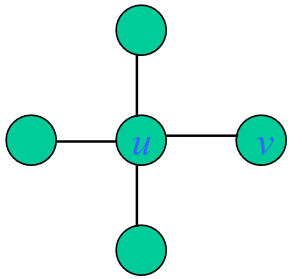
\includegraphics[width=0.4\textwidth]{10 ott/graph.png}
\end{figure}

\subsection{Notazione \textit{o} Piccolo}
Definiamo $f(n) = o(g(n))$ se $\lim_{n \to \infty} \frac{f(n)}{g(n)} = 0$.
\\
\textbf{Nota:}
$o(g(n)) \subset O(g(n))$
\subsection{Notazione Omega Piccolo}
Definiamo $f(n) = \omega(g(n))$ se $\lim_{n \to \infty} \frac{f(n)}{g(n)} = \infty$.
\\
\textbf{Nota:}
$\omega(g(n)) \subset \Omega(g(n))$
\subsection{Alcune Proprietà}

\begin{itemize}
    \item $f(\Omega) = O(g(n))$ se e solo se $g(n) = \Omega(f(n))$.
    \item $f(n) = o(g(n))$ se e solo se $g(n) = \omega(f(n))$.
\end{itemize}

\section{Alcuni Limiti Notevoli}

\subsection{Polinomi}
Se $P(n) = a_d \cdot n^d + a_{d-1} \cdot n^{d-1} + \ldots + a_0$: \\
\begin{align}
    P(n) &= \Theta(n^d) \\
    P(n) &= O(n^d) \\
    P(n) &= \Omega(n^d)
\end{align}

\subsection{Esponenziali}
Se $f(n) = a^n$:\\
\begin{align}
    a^n &= \omega(n^d) \\
    a^n &= \Omega(n^d)
\end{align}

\subsection{Logaritmi}
Se $f(n) = \log_b(n)$:
\begin{align} \\
    \log_b(n)^c &= o(n^d) \\
    \log_b(n)^c &= O(n^d)
\end{align}

\subsection{Fattoriali}
Se $f(n) = n!$:
\begin{align} \\
    n! &= o(n^n) \\
    n! &= \omega(a^n)
\end{align}

\section{Velocità delle Funzioni Composte}

\begin{itemize}
    \item Date $f(n)$ e $g(n)$, la velocità della funzione $f(n) + g(n)$ è la velocità della più veloce tra $f(n)$ e $g(n)$.
    \item Date $f(n)$ e $g(n)$, la velocità della funzione $f(n) \cdot g(n)$ è la velocità di $f(n)$ "più" la velocità di $g(n)$.
    \item Date $f(n)$ e $g(n)$, la velocità della funzione $f(n) / g(n)$ è la velocità di $f(n)$ "meno" la velocità di $g(n)$.
\end{itemize}

\section{Usare la Notazione Asintotica nelle Analisi}

\subsection{Analisi della Complessità di fibonacci3}
\begin{algorithm}
\caption{fibonacci3}
\begin{algorithmic}[1]
\Function{fibonacci3}{intero $n$} $\rightarrow$ intero
  \State Sia $Fib$ un array di $n$ interi
  \State $Fib[1] = 1; Fib[2] = 1$
  \For{$i = 3$ to $n$}
    \State $Fib[i] = Fib[i-1] + Fib[i-2]$
  \EndFor
  \State \Return $Fib[n]$
\EndFunction
\end{algorithmic}
\end{algorithm}
$T(n)$ rappresenta la complessità computazionale nel caso peggiore con input $n$. \\ 
$c_j$ rappresenta il numero di passi elementari eseguiti su una RAM quando è eseguita la linea di codice $j$.

\subsection{Upper Bound}
\begin{itemize}
    \item Linee 1, 3, 5 eseguite una sola volta.
    \item Linee 3 e 4 eseguite al più $n$ volte.
\end{itemize}

$T(n) \leq c_1 + c_3 + c_5 + (c_3 + c_4) \cdot n = \Theta(n)$

$\Rightarrow T(n) = O(n)$

\subsection{Lower Bound}
\begin{itemize}
    \item La linea 4 è eseguita almeno $n-3$ volte.
\end{itemize}

$T(n) \geq c_4 \cdot (n-3) = \Theta(n)$

$\Rightarrow T(n) = \Omega(n)$

$\Rightarrow T(n) = O(n)$ e $T(n) = \Omega(n) \Rightarrow T(n) = \Theta(n)$

\section{Perché è una grande idea la notazione asintotica:}
\begin{itemize}
    \item Misura indipendente dall'implementazione dell'algoritmo e dalla macchina reale.
    \item I dettagli nascosti sono poco rilevanti per $n$ molto grandi.
    \item Un'analisi dettagliata del numero di passi realmente eseguiti sarebbe difficile, noiosa e non direbbe molto di più.
    \item Descrive bene in pratica la velocità degli algoritmi.
\end{itemize}


\end{document}